% Options for packages loaded elsewhere
\PassOptionsToPackage{unicode}{hyperref}
\PassOptionsToPackage{hyphens}{url}
%
\documentclass[
]{article}
\title{First steps with ggplot2}
\author{Group 4: Alex Tai, Momo Mbarek, Zhang Zichen}
\date{16/02/2022}

\usepackage{amsmath,amssymb}
\usepackage{lmodern}
\usepackage{iftex}
\ifPDFTeX
  \usepackage[T1]{fontenc}
  \usepackage[utf8]{inputenc}
  \usepackage{textcomp} % provide euro and other symbols
\else % if luatex or xetex
  \usepackage{unicode-math}
  \defaultfontfeatures{Scale=MatchLowercase}
  \defaultfontfeatures[\rmfamily]{Ligatures=TeX,Scale=1}
\fi
% Use upquote if available, for straight quotes in verbatim environments
\IfFileExists{upquote.sty}{\usepackage{upquote}}{}
\IfFileExists{microtype.sty}{% use microtype if available
  \usepackage[]{microtype}
  \UseMicrotypeSet[protrusion]{basicmath} % disable protrusion for tt fonts
}{}
\makeatletter
\@ifundefined{KOMAClassName}{% if non-KOMA class
  \IfFileExists{parskip.sty}{%
    \usepackage{parskip}
  }{% else
    \setlength{\parindent}{0pt}
    \setlength{\parskip}{6pt plus 2pt minus 1pt}}
}{% if KOMA class
  \KOMAoptions{parskip=half}}
\makeatother
\usepackage{xcolor}
\IfFileExists{xurl.sty}{\usepackage{xurl}}{} % add URL line breaks if available
\IfFileExists{bookmark.sty}{\usepackage{bookmark}}{\usepackage{hyperref}}
\hypersetup{
  pdftitle={First steps with ggplot2},
  pdfauthor={Group 4: Alex Tai, Momo Mbarek, Zhang Zichen},
  hidelinks,
  pdfcreator={LaTeX via pandoc}}
\urlstyle{same} % disable monospaced font for URLs
\usepackage[margin=1in]{geometry}
\usepackage{color}
\usepackage{fancyvrb}
\newcommand{\VerbBar}{|}
\newcommand{\VERB}{\Verb[commandchars=\\\{\}]}
\DefineVerbatimEnvironment{Highlighting}{Verbatim}{commandchars=\\\{\}}
% Add ',fontsize=\small' for more characters per line
\usepackage{framed}
\definecolor{shadecolor}{RGB}{248,248,248}
\newenvironment{Shaded}{\begin{snugshade}}{\end{snugshade}}
\newcommand{\AlertTok}[1]{\textcolor[rgb]{0.94,0.16,0.16}{#1}}
\newcommand{\AnnotationTok}[1]{\textcolor[rgb]{0.56,0.35,0.01}{\textbf{\textit{#1}}}}
\newcommand{\AttributeTok}[1]{\textcolor[rgb]{0.77,0.63,0.00}{#1}}
\newcommand{\BaseNTok}[1]{\textcolor[rgb]{0.00,0.00,0.81}{#1}}
\newcommand{\BuiltInTok}[1]{#1}
\newcommand{\CharTok}[1]{\textcolor[rgb]{0.31,0.60,0.02}{#1}}
\newcommand{\CommentTok}[1]{\textcolor[rgb]{0.56,0.35,0.01}{\textit{#1}}}
\newcommand{\CommentVarTok}[1]{\textcolor[rgb]{0.56,0.35,0.01}{\textbf{\textit{#1}}}}
\newcommand{\ConstantTok}[1]{\textcolor[rgb]{0.00,0.00,0.00}{#1}}
\newcommand{\ControlFlowTok}[1]{\textcolor[rgb]{0.13,0.29,0.53}{\textbf{#1}}}
\newcommand{\DataTypeTok}[1]{\textcolor[rgb]{0.13,0.29,0.53}{#1}}
\newcommand{\DecValTok}[1]{\textcolor[rgb]{0.00,0.00,0.81}{#1}}
\newcommand{\DocumentationTok}[1]{\textcolor[rgb]{0.56,0.35,0.01}{\textbf{\textit{#1}}}}
\newcommand{\ErrorTok}[1]{\textcolor[rgb]{0.64,0.00,0.00}{\textbf{#1}}}
\newcommand{\ExtensionTok}[1]{#1}
\newcommand{\FloatTok}[1]{\textcolor[rgb]{0.00,0.00,0.81}{#1}}
\newcommand{\FunctionTok}[1]{\textcolor[rgb]{0.00,0.00,0.00}{#1}}
\newcommand{\ImportTok}[1]{#1}
\newcommand{\InformationTok}[1]{\textcolor[rgb]{0.56,0.35,0.01}{\textbf{\textit{#1}}}}
\newcommand{\KeywordTok}[1]{\textcolor[rgb]{0.13,0.29,0.53}{\textbf{#1}}}
\newcommand{\NormalTok}[1]{#1}
\newcommand{\OperatorTok}[1]{\textcolor[rgb]{0.81,0.36,0.00}{\textbf{#1}}}
\newcommand{\OtherTok}[1]{\textcolor[rgb]{0.56,0.35,0.01}{#1}}
\newcommand{\PreprocessorTok}[1]{\textcolor[rgb]{0.56,0.35,0.01}{\textit{#1}}}
\newcommand{\RegionMarkerTok}[1]{#1}
\newcommand{\SpecialCharTok}[1]{\textcolor[rgb]{0.00,0.00,0.00}{#1}}
\newcommand{\SpecialStringTok}[1]{\textcolor[rgb]{0.31,0.60,0.02}{#1}}
\newcommand{\StringTok}[1]{\textcolor[rgb]{0.31,0.60,0.02}{#1}}
\newcommand{\VariableTok}[1]{\textcolor[rgb]{0.00,0.00,0.00}{#1}}
\newcommand{\VerbatimStringTok}[1]{\textcolor[rgb]{0.31,0.60,0.02}{#1}}
\newcommand{\WarningTok}[1]{\textcolor[rgb]{0.56,0.35,0.01}{\textbf{\textit{#1}}}}
\usepackage{graphicx}
\makeatletter
\def\maxwidth{\ifdim\Gin@nat@width>\linewidth\linewidth\else\Gin@nat@width\fi}
\def\maxheight{\ifdim\Gin@nat@height>\textheight\textheight\else\Gin@nat@height\fi}
\makeatother
% Scale images if necessary, so that they will not overflow the page
% margins by default, and it is still possible to overwrite the defaults
% using explicit options in \includegraphics[width, height, ...]{}
\setkeys{Gin}{width=\maxwidth,height=\maxheight,keepaspectratio}
% Set default figure placement to htbp
\makeatletter
\def\fps@figure{htbp}
\makeatother
\setlength{\emergencystretch}{3em} % prevent overfull lines
\providecommand{\tightlist}{%
  \setlength{\itemsep}{0pt}\setlength{\parskip}{0pt}}
\setcounter{secnumdepth}{-\maxdimen} % remove section numbering
\ifLuaTeX
  \usepackage{selnolig}  % disable illegal ligatures
\fi

\begin{document}
\maketitle

We need to load the following packages.

\begin{Shaded}
\begin{Highlighting}[]
\FunctionTok{library}\NormalTok{(ggplot2)}
\FunctionTok{library}\NormalTok{(tidyverse)}
\end{Highlighting}
\end{Shaded}

\hypertarget{exercise-1}{%
\subsubsection{1. Exercise 1}\label{exercise-1}}

\begin{enumerate}
\def\labelenumi{(\alph{enumi})}
\item
  Import the CSV file as a tibble and remove unwanted columns

\begin{Shaded}
\begin{Highlighting}[]
\NormalTok{titanic\_1 }\OtherTok{\textless{}{-}} \FunctionTok{read\_csv}\NormalTok{(}\StringTok{"titanic.csv"}\NormalTok{, }\AttributeTok{show\_col\_types =} \ConstantTok{FALSE}\NormalTok{)}

\CommentTok{\# remove unwanted columns}
\NormalTok{titanic\_1 }\OtherTok{\textless{}{-}}\NormalTok{ titanic\_1[, }\FunctionTok{c}\NormalTok{(}\StringTok{"class"}\NormalTok{, }\StringTok{"survived"}\NormalTok{)]}
\end{Highlighting}
\end{Shaded}
\item
  Make a bar plot of passengers by class

\begin{Shaded}
\begin{Highlighting}[]
  \FunctionTok{ggplot}\NormalTok{(titanic\_1, }\FunctionTok{aes}\NormalTok{(}\AttributeTok{x =}\NormalTok{ class)) }\SpecialCharTok{+}
  \FunctionTok{geom\_bar}\NormalTok{() }\SpecialCharTok{+} \FunctionTok{labs}\NormalTok{(}
    \AttributeTok{title =} \StringTok{"Passengers in Titanic by class"}\NormalTok{,}
    \AttributeTok{caption =} \StringTok{"Source: Encyclopedia Titanica"}\NormalTok{,}
    \AttributeTok{x =} \StringTok{"Class"}\NormalTok{,}
    \AttributeTok{y =} \StringTok{"Number of passengers"}
\NormalTok{    )}
\end{Highlighting}
\end{Shaded}

  \begin{center}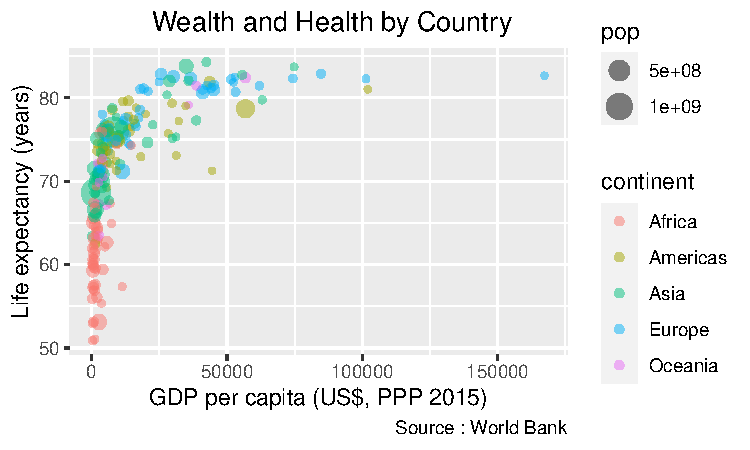
\includegraphics[width=0.6\linewidth]{Grp4_first_steps_with_ggplot2_files/figure-latex/unnamed-chunk-3-1} \end{center}
\item
  Make a side-by-side bar plot to visualise the dependence of the number
  of survivors on their class

\begin{Shaded}
\begin{Highlighting}[]
  \FunctionTok{ggplot}\NormalTok{(titanic\_1, }\FunctionTok{aes}\NormalTok{(}\AttributeTok{fill =}\NormalTok{ survived, }\AttributeTok{x =}\NormalTok{ class)) }\SpecialCharTok{+}
  \FunctionTok{geom\_bar}\NormalTok{(}\AttributeTok{position =} \StringTok{"dodge"}\NormalTok{) }\SpecialCharTok{+} \CommentTok{\# make the bar plot side{-}by{-}side}
  \FunctionTok{labs}\NormalTok{(}
    \AttributeTok{title =} \StringTok{"Passengers in Titanic by class"}\NormalTok{,}
    \AttributeTok{caption =} \StringTok{"Source: Encyclopedia Titanica"}\NormalTok{,}
    \AttributeTok{x =} \StringTok{"Class"}\NormalTok{,}
    \AttributeTok{y =} \StringTok{"Number of passengers"}
\NormalTok{    )}
\end{Highlighting}
\end{Shaded}

  \begin{center}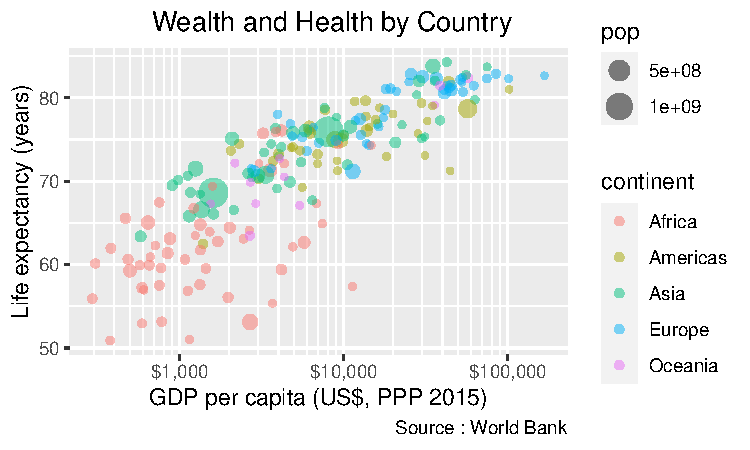
\includegraphics[width=0.7\linewidth]{Grp4_first_steps_with_ggplot2_files/figure-latex/unnamed-chunk-4-1} \end{center}
\item
  Turn the built-in data set Titanic into a tibble

\begin{Shaded}
\begin{Highlighting}[]
\NormalTok{  titanic\_2 }\OtherTok{\textless{}{-}}
  \FunctionTok{apply}\NormalTok{(Titanic, }\FunctionTok{c}\NormalTok{(}\DecValTok{1}\NormalTok{, }\DecValTok{4}\NormalTok{), sum) }\SpecialCharTok{|}\ErrorTok{\textgreater{}}
  \FunctionTok{as\_tibble}\NormalTok{(}\AttributeTok{rownames =} \StringTok{"class"}\NormalTok{) }\SpecialCharTok{|}\ErrorTok{\textgreater{}}
  \FunctionTok{rename}\NormalTok{(}\AttributeTok{died =} \StringTok{"No"}\NormalTok{, }\AttributeTok{survived =} \StringTok{"Yes"}\NormalTok{)}
\end{Highlighting}
\end{Shaded}
\item
  Add a column to \texttt{titanic\_2} with the total number of
  passengers in each class

\begin{Shaded}
\begin{Highlighting}[]
\NormalTok{  titanic\_2}\SpecialCharTok{$}\NormalTok{total }\OtherTok{\textless{}{-}}\NormalTok{ titanic\_2}\SpecialCharTok{$}\NormalTok{died }\SpecialCharTok{+}\NormalTok{ titanic\_2}\SpecialCharTok{$}\NormalTok{survived}
\end{Highlighting}
\end{Shaded}

  We can see that for \texttt{titanic\_1}, each passenger is a single
  data entry which indicates their individual class and survival status.
  Meanwhile in \texttt{titanic\_2}, there are no entries for individual
  passengers, and only the total number of passengers, the number of
  survived passengers, and the number of passengers who died in each
  class is included.
\item
  Redo the plot in (b) with \texttt{titanic\_2}

\begin{Shaded}
\begin{Highlighting}[]
  \FunctionTok{ggplot}\NormalTok{(titanic\_2, }\FunctionTok{aes}\NormalTok{(}\AttributeTok{x =}\NormalTok{ class, }\AttributeTok{y =}\NormalTok{ total)) }\SpecialCharTok{+}
  \FunctionTok{geom\_bar}\NormalTok{(}\AttributeTok{stat =} \StringTok{"identity"}\NormalTok{) }\SpecialCharTok{+}
  \FunctionTok{labs}\NormalTok{(}
    \AttributeTok{title =} \StringTok{"Passengers in Titanic by class"}\NormalTok{,}
    \AttributeTok{caption =} \StringTok{"Source: Encyclopedia Titanica"}\NormalTok{,}
    \AttributeTok{x =} \StringTok{"Class"}\NormalTok{,}
    \AttributeTok{y =} \StringTok{"Number of passengers"}
\NormalTok{    )}
\end{Highlighting}
\end{Shaded}

  \begin{center}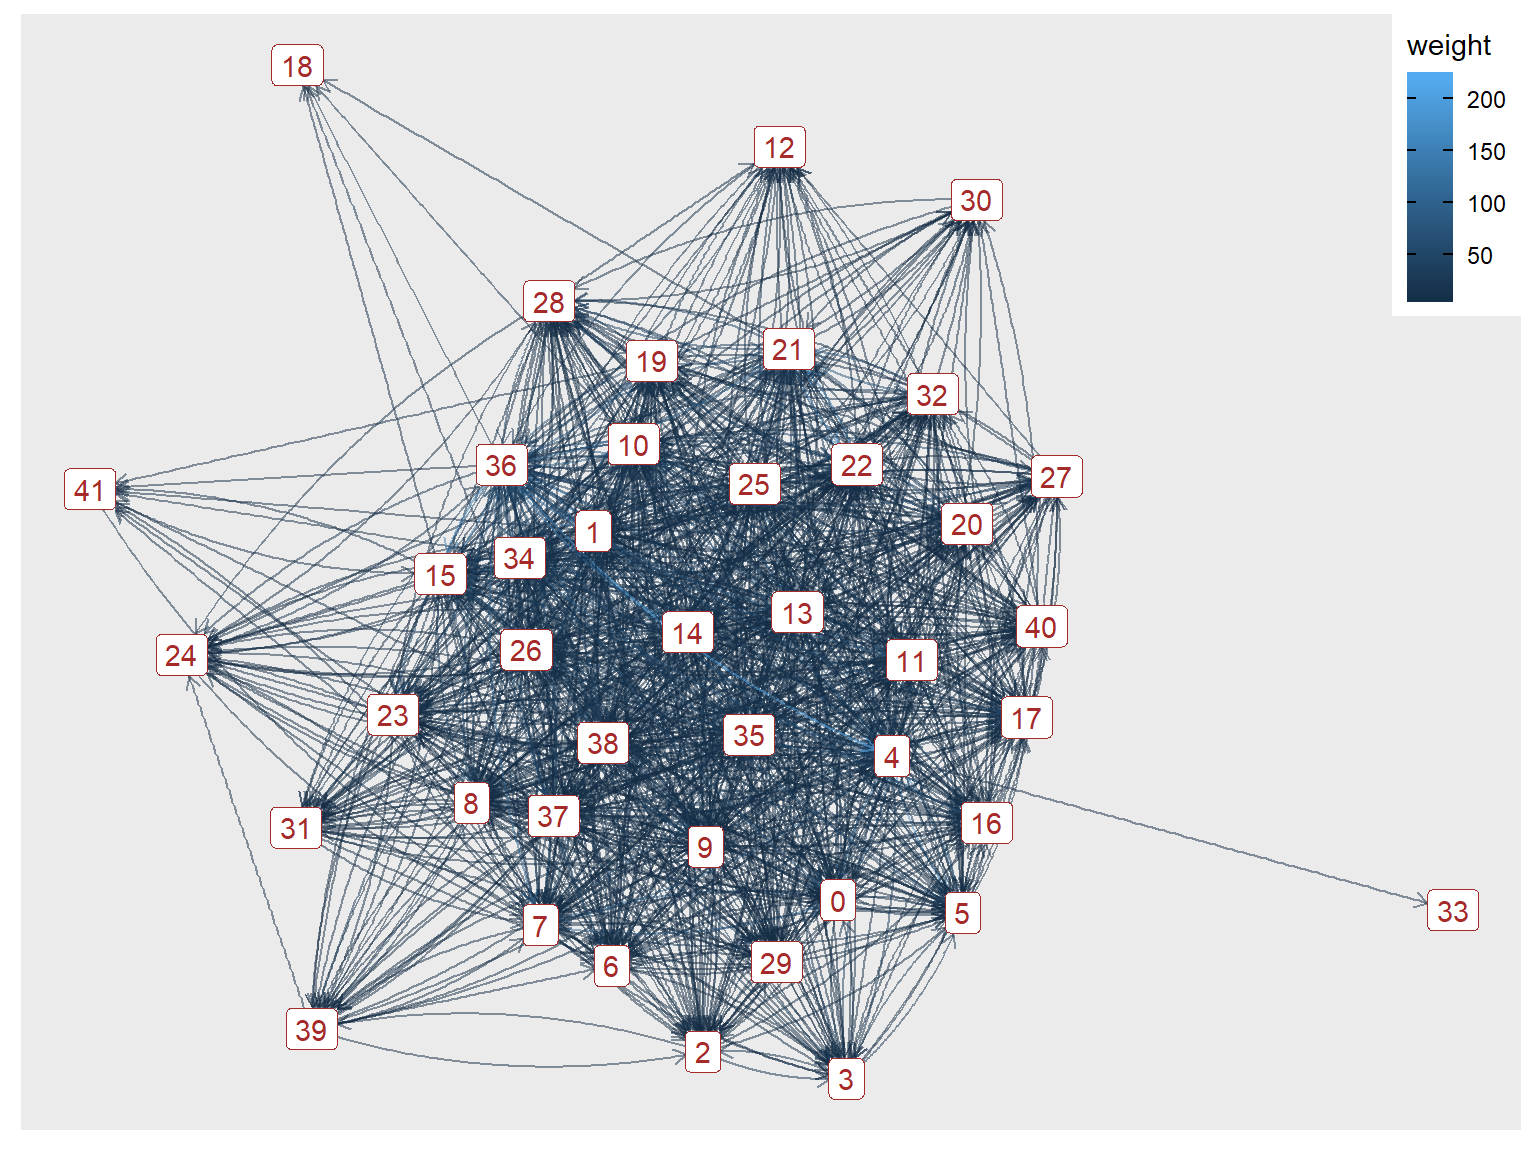
\includegraphics[width=0.6\linewidth]{Grp4_first_steps_with_ggplot2_files/figure-latex/unnamed-chunk-7-1} \end{center}
\end{enumerate}

\hypertarget{exercise-2}{%
\subsubsection{2. Exercise 2}\label{exercise-2}}

\begin{enumerate}
\def\labelenumi{(\alph{enumi})}
\item
  Change the column Expt to be a factor instead of an integer

\begin{Shaded}
\begin{Highlighting}[]
  \CommentTok{\# load the data}
  \FunctionTok{data}\NormalTok{(morley)}

  \CommentTok{\# turn the Expt column into a factor}
\NormalTok{  morley}\SpecialCharTok{$}\NormalTok{Expt }\OtherTok{\textless{}{-}} \FunctionTok{factor}\NormalTok{(morley}\SpecialCharTok{$}\NormalTok{Expt)}
\end{Highlighting}
\end{Shaded}
\item
  Make a scatter plot of Speed (y-axis) versus experiment number
  (x-axis)

\begin{Shaded}
\begin{Highlighting}[]
  \FunctionTok{ggplot}\NormalTok{(morley, }\FunctionTok{aes}\NormalTok{(}\AttributeTok{x =}\NormalTok{ Expt, }\AttributeTok{y =}\NormalTok{ Speed)) }\SpecialCharTok{+} 
  \FunctionTok{geom\_point}\NormalTok{(}
    \FunctionTok{aes}\NormalTok{(}\AttributeTok{colour =}\NormalTok{ Expt, }
        \AttributeTok{show.legend =} \ConstantTok{FALSE}\NormalTok{)) }\SpecialCharTok{+}
  \FunctionTok{labs}\NormalTok{(}
    \AttributeTok{title =} \StringTok{"Measured speed in different experiments"}\NormalTok{,}
    \AttributeTok{x =} \StringTok{"Experiment number"}\NormalTok{,}
    \AttributeTok{y =} \StringTok{"Measured speed of light (km/s)"}\NormalTok{)}
\end{Highlighting}
\end{Shaded}

\begin{verbatim}
## Warning: Ignoring unknown aesthetics: show.legend
\end{verbatim}

  \begin{center}\includegraphics[width=0.6\linewidth]{Grp4_first_steps_with_ggplot2_files/figure-latex/unnamed-chunk-9-1} \end{center}
\item
  Make another scatter plot with geom\_jitter()

\begin{Shaded}
\begin{Highlighting}[]
  \FunctionTok{ggplot}\NormalTok{(morley, }\FunctionTok{aes}\NormalTok{(Expt, Speed)) }\SpecialCharTok{+}
\FunctionTok{geom\_jitter}\NormalTok{(}
  \AttributeTok{width =} \FloatTok{0.2}\NormalTok{,}
  \AttributeTok{height =} \DecValTok{0}\NormalTok{,}
  \AttributeTok{size =} \FloatTok{0.8}\NormalTok{,}
  \FunctionTok{aes}\NormalTok{(}\AttributeTok{colour =}\NormalTok{ Expt),}
  \AttributeTok{show.legend =} \ConstantTok{FALSE}
\NormalTok{) }\SpecialCharTok{+}
\FunctionTok{labs}\NormalTok{(}
  \AttributeTok{title =} \StringTok{"Measured speed in different experiments"}\NormalTok{,}
  \AttributeTok{x =} \StringTok{"Experiment number"}\NormalTok{,}
  \AttributeTok{y =} \StringTok{"Measured speed of light (km/s)"}
\NormalTok{)}
\end{Highlighting}
\end{Shaded}

  \begin{center}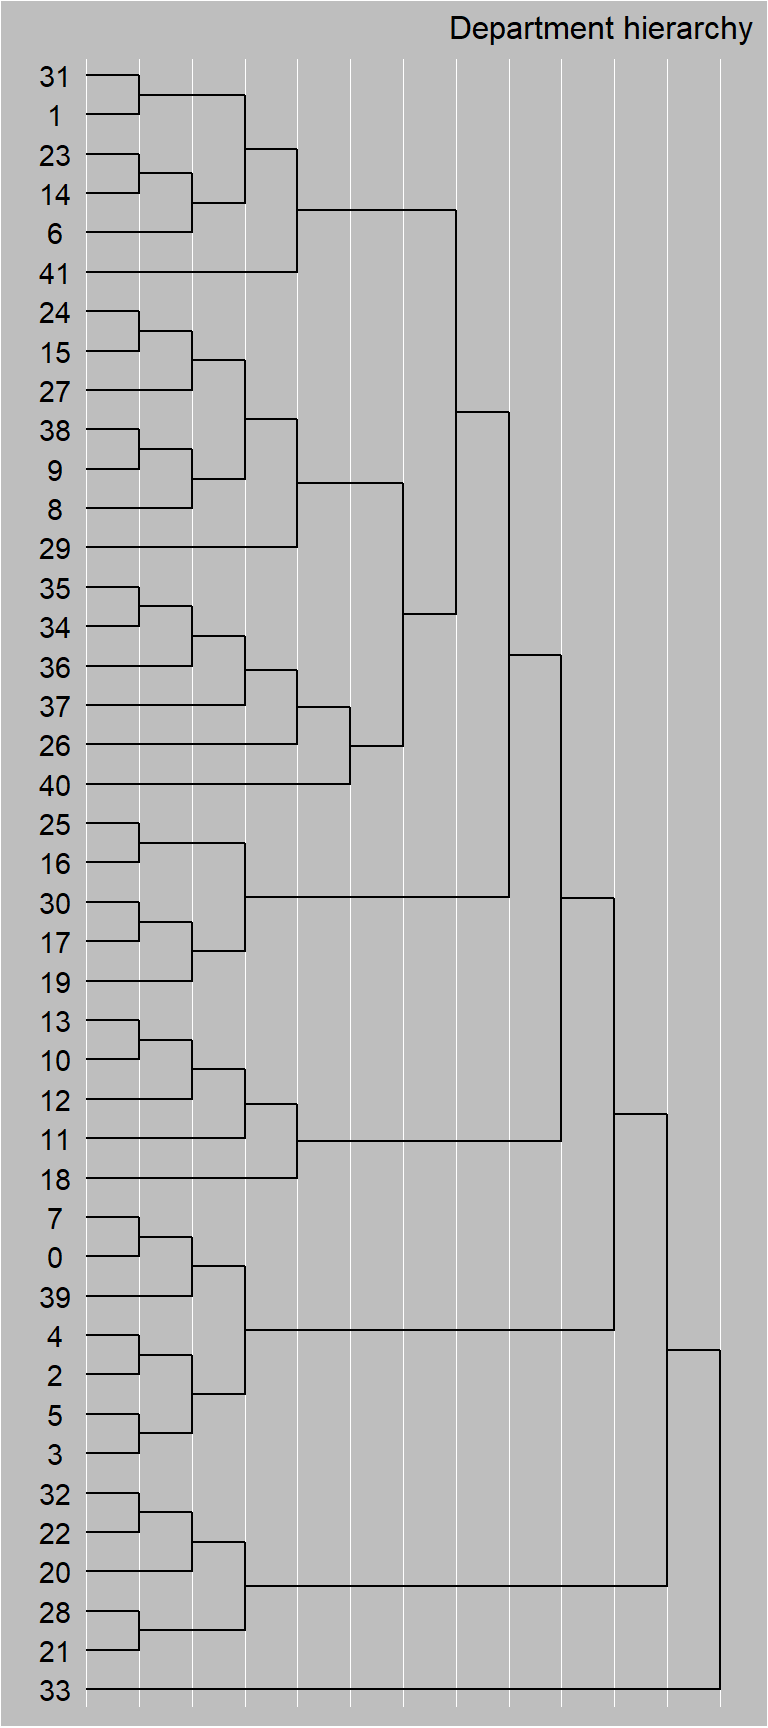
\includegraphics[width=0.6\linewidth]{Grp4_first_steps_with_ggplot2_files/figure-latex/unnamed-chunk-10-1} \end{center}

  The default width value needs to be changed for \texttt{geom\_jitter}
  to make data that belong one experiment clearly distinctive from data
  that belong to other experiments. If this is not done, data points of
  different experiments would cluster together, making it difficult to
  tell which point belongs to which experiment and draw insights from
  the plot.
\item
  Briefly describe what a box plot shows in general
\end{enumerate}

\begin{itemize}
\tightlist
\item
  A box plot shows five key statistics of continuous variables grouped
  by a category.
\item
  The bottom and top of the box shows the 25th and 75th percentiles of
  some continuous data, while the line in the box shows the median.
\item
  The end of the two whiskers show the minimum and maximum respectively.
\item
  Any point that lays outside the whiskers is considered an outlier.
\end{itemize}

\begin{enumerate}
\def\labelenumi{(\alph{enumi})}
\setcounter{enumi}{4}
\tightlist
\item
  Make a box plot of the measured speeds with one box for each
  experiment
\end{enumerate}

\begin{Shaded}
\begin{Highlighting}[]
  \FunctionTok{ggplot}\NormalTok{(morley, }\FunctionTok{aes}\NormalTok{(Expt, Speed)) }\SpecialCharTok{+} 
  \FunctionTok{geom\_boxplot}\NormalTok{() }\SpecialCharTok{+}
  \FunctionTok{labs}\NormalTok{(}
    \AttributeTok{title =} \StringTok{"Speed of light in different experiments"}\NormalTok{,}
    \AttributeTok{x =} \StringTok{"Experiment number"}\NormalTok{,}
    \AttributeTok{y =} \StringTok{"Measured speed of light (km/s)"}
\NormalTok{  )}
\end{Highlighting}
\end{Shaded}

\begin{center}\includegraphics[width=0.6\linewidth]{Grp4_first_steps_with_ggplot2_files/figure-latex/unnamed-chunk-11-1} \end{center}

\begin{enumerate}
\def\labelenumi{(\alph{enumi})}
\setcounter{enumi}{5}
\tightlist
\item
  Make a violin plot with one violin for each experiment number
\end{enumerate}

\begin{Shaded}
\begin{Highlighting}[]
  \FunctionTok{ggplot}\NormalTok{(morley, }\FunctionTok{aes}\NormalTok{(Expt, Speed)) }\SpecialCharTok{+} 
  \FunctionTok{geom\_violin}\NormalTok{() }\SpecialCharTok{+}
  \FunctionTok{labs}\NormalTok{(}
    \AttributeTok{title =} \StringTok{"Speed of light in different experiments"}\NormalTok{,}
    \AttributeTok{x =} \StringTok{"Experiment number"}\NormalTok{,}
    \AttributeTok{y =} \StringTok{"Measured speed of light (km/s)"}
\NormalTok{  )}
\end{Highlighting}
\end{Shaded}

\begin{center}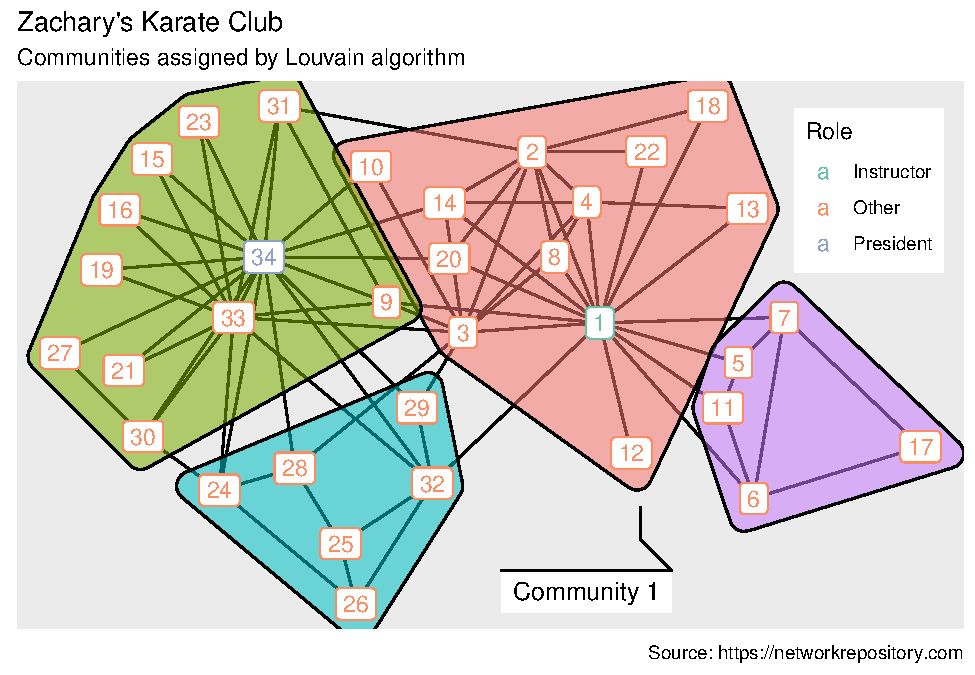
\includegraphics[width=0.6\linewidth]{Grp4_first_steps_with_ggplot2_files/figure-latex/unnamed-chunk-12-1} \end{center}

\begin{enumerate}
\def\labelenumi{(\alph{enumi})}
\setcounter{enumi}{6}
\tightlist
\item
  What is the advantage of a violin plot compared to a box plot? What is
  the disadvantage?
\end{enumerate}

\begin{itemize}
\item
  A violin plot is more advantageous than a box plot in showing the
  probability densities distributed over the entire data range. This is
  useful when we are interested in the detailed data distribution. If
  the data is bimodal, for instance, a violin plot woudl allow us to see
  the different modes while a box plot would not.
\item
  One disadvantage of a violin plot is that it does not show the
  interquartile range or the median precisely. This would make it harder
  to compare those characteristics accross different data groups.
\end{itemize}

\begin{enumerate}
\def\labelenumi{(\alph{enumi})}
\setcounter{enumi}{7}
\tightlist
\item
  Make a faceted plot with one histogram for each experiment's speed
  distribution
\end{enumerate}

\begin{Shaded}
\begin{Highlighting}[]
  \FunctionTok{ggplot}\NormalTok{(morley, }\FunctionTok{aes}\NormalTok{(}\AttributeTok{x =}\NormalTok{ Speed)) }\SpecialCharTok{+}
  \FunctionTok{geom\_histogram}\NormalTok{(}\AttributeTok{binwidth =} \DecValTok{25}\NormalTok{) }\SpecialCharTok{+} \CommentTok{\# change to a suitable bin width}
  \FunctionTok{facet\_grid}\NormalTok{(Expt }\SpecialCharTok{\textasciitilde{}}\NormalTok{ .) }\SpecialCharTok{+} \CommentTok{\# make stacked histograms for each experiment number}
  \FunctionTok{labs}\NormalTok{(}
    \AttributeTok{title =} \StringTok{"Speed distribution of each experiment"}\NormalTok{,}
    \AttributeTok{x =} \StringTok{"Measured speed of light (km/s)"}\NormalTok{,}
    \AttributeTok{y =} \StringTok{"Count"}
\NormalTok{  )}
\end{Highlighting}
\end{Shaded}

\begin{center}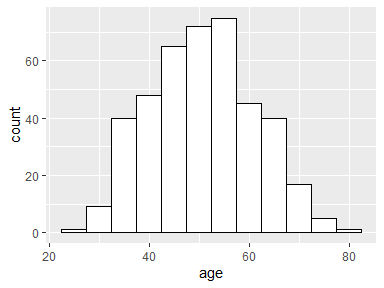
\includegraphics[width=0.47\linewidth]{Grp4_first_steps_with_ggplot2_files/figure-latex/unnamed-chunk-13-1} \end{center}

\begin{enumerate}
\def\labelenumi{(\roman{enumi})}
\tightlist
\item
  Show the speed distribution of each experiment as a frequency polygon.
  Do not use faceting.
\end{enumerate}

\begin{Shaded}
\begin{Highlighting}[]
  \FunctionTok{ggplot}\NormalTok{(morley, }\FunctionTok{aes}\NormalTok{(Speed, }\AttributeTok{colour =}\NormalTok{ Expt)) }\SpecialCharTok{+} 
  \FunctionTok{geom\_freqpoly}\NormalTok{(}\AttributeTok{binwidth =} \DecValTok{40}\NormalTok{) }\SpecialCharTok{+} 
  \FunctionTok{labs}\NormalTok{(}
    \AttributeTok{title =} \StringTok{"Speed distribution of each experiment"}\NormalTok{,}
    \AttributeTok{x =} \StringTok{"Measured speed of light (km/s)"}\NormalTok{,}
    \AttributeTok{y =} \StringTok{"Count"}\NormalTok{,}
    \AttributeTok{colour =} \StringTok{"Experiment number"}
\NormalTok{  )}
\end{Highlighting}
\end{Shaded}

\begin{center}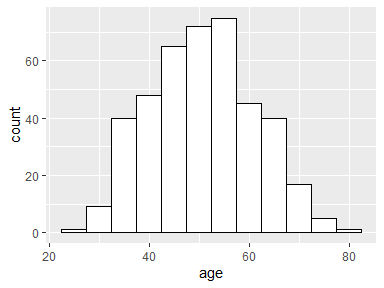
\includegraphics[width=0.6\linewidth]{Grp4_first_steps_with_ggplot2_files/figure-latex/unnamed-chunk-14-1} \end{center}

\begin{enumerate}
\def\labelenumi{(\alph{enumi})}
\setcounter{enumi}{9}
\tightlist
\item
  What is the advantage of using non-faceted frequency polygons compared
  to faceted histograms? What is the disadvantage?
\end{enumerate}

\begin{itemize}
\item
  The advantage of using frequency polygons instead of faceted
  histograms is that it saves space. Physically, the plot takes one set
  of axis and lables, and represents the information of different
  subgroups close to each other for ease of comparison.
\item
  The disadvantage of using frequency polygons is readability. With the
  number of lines exceeding 3 or 4, is becomes increasingly difficult to
  `follow' along each separate line as their slopes change. Plotting the
  lines on top of each other is also an area of concern which makes the
  plot less readable.
\end{itemize}

\end{document}
